\documentclass[11pt]{beamer}
%\usetheme{metropolis}
\usetheme{Madrid}
%\usetheme{Frankfurt}
%\usecolortheme{dolphin}


\usepackage[utf8]{inputenc}
\usepackage[spanish]{babel}
\selectlanguage{spanish}


\usepackage{amsmath}
\usepackage{amsfonts}
\usepackage{amssymb}
\usepackage{graphicx}
\usepackage{media9}
\usepackage{movie15}
\usepackage{listings}
\usepackage{color}
\usepackage{fancyvrb}


\definecolor{pblue}{rgb}{0.13,0.13,1}
\definecolor{pgreen}{rgb}{0,0.5,0}
\definecolor{pred}{rgb}{0.9,0,0}
\definecolor{pgrey}{rgb}{0.46,0.45,0.48}
\lstset{
language=Java,
commentstyle=\color{pgreen},
keywordstyle=\color{pblue},
stringstyle=\color{pred},
basicstyle=\small\sffamily,
numbers=left,
numberstyle=\tiny,
frame=tb,
columns=fullflexible,
showstringspaces=false
}

\definecolor{maroon}{rgb}{0.5,0,0}
\definecolor{darkgreen}{rgb}{0,0.5,0}
\lstdefinelanguage{XML}
{
  basicstyle=\ttfamily,
  morestring=[s]{"}{"},
  morecomment=[s]{?}{?},
  morecomment=[s]{!--}{--},
  commentstyle=\color{darkgreen},
  moredelim=[s][\color{black}]{>}{<},
  moredelim=[s][\color{red}]{\ }{=},
  stringstyle=\color{blue},
  identifierstyle=\color{maroon},
  numbers=none
}

\author{Javier Fuentes Muñoz \\ \texttt{j.fuentes06@ufromail.cl}}

\title{MINERÍA DE DATOS}
\subtitle{PARA LOGS DE ALMA COMMON SOFTWARE} 
%\setbeamercovered{transparent} 

%\setbeamertemplate{navigation symbols}{} 
\titlegraphic{\hfill
\includegraphics[height=1.5cm]{logo}}

\institute{Universidad de La Frontera} 
\date{\today} 

\begin{document}

\begin{frame}
\titlepage
\end{frame}

\section{Acerca de alma}

\begin{frame}{Acerca de ALMA}

\centering\textbf{Colaboración ALMA-UFRO}
\vfill
		\centering
		
\includegraphics[height=3cm]{logo}
		\hspace{1cm}
		
\includegraphics[height=3cm]{alma-logo}
	
\end{frame}

\begin{frame}{Acerca de ALMA}
	\centering
	\includegraphics[height=6cm]{alma}
	\vfill
	\textit{...explorando nuestros orígenes cósmicos...}
	
\end{frame}

\section{Problemática general}

\begin{frame}{Problemática general}
	\begin{itemize}
		\item Software distribuido
		\item Altamente complejo
		\item Grandes volumenes de logs del sistema
		\item Análisis de los datos
	\end{itemize}
\end{frame}

\section{Objetivos}
\begin{frame}{Objetivo General}
\begin{itemize}
	\item Aplicar metodologías CRISP para generar un modelo de análisis de los LOGS de ACS.
\end{itemize}	
\end{frame}

\begin{frame}{Objetivos Específicos}
	

\begin{itemize}	
	\item Identificar un problema relevante para ALMA y que pueda ser abordado analizando los logs del sistema ACS.
	\item Diseñar una metodología basada en CRISP para abordar la problemática identificada.
	\item Crear un prototipo de pre-procesamiento del log de ACS.
\end{itemize}

\end{frame}
\section{Antecedentes}

\begin{frame}{ACS}
	\begin{itemize}
		\item Infraestructura distribuida
		\item CORBA
		\item Sistema de \texttt{logging}
	\end{itemize}
\end{frame}

\begin{frame}{Infraestructura distribuida}
\begin{figure}
\centering
	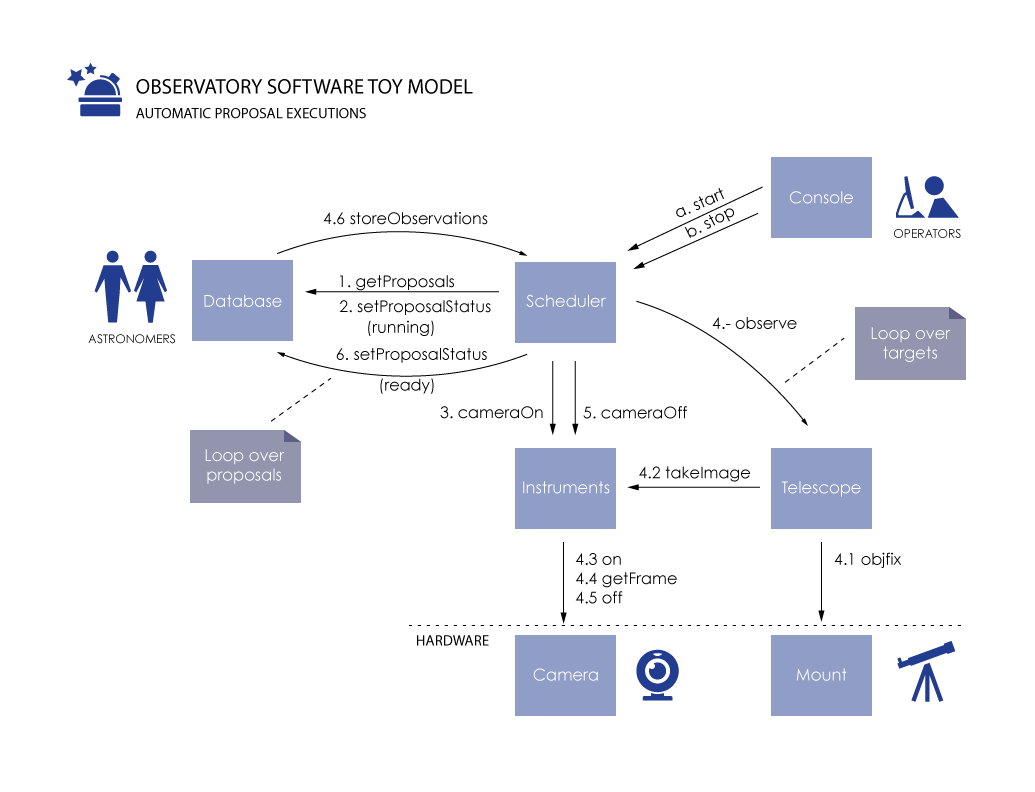
\includegraphics[height=6.8cm]{alma_toy_model}
\caption{ALMA-ACS Toy Model}
\end{figure}
\end{frame}


\begin{frame}{CORBA}
\begin{figure}
\centering
	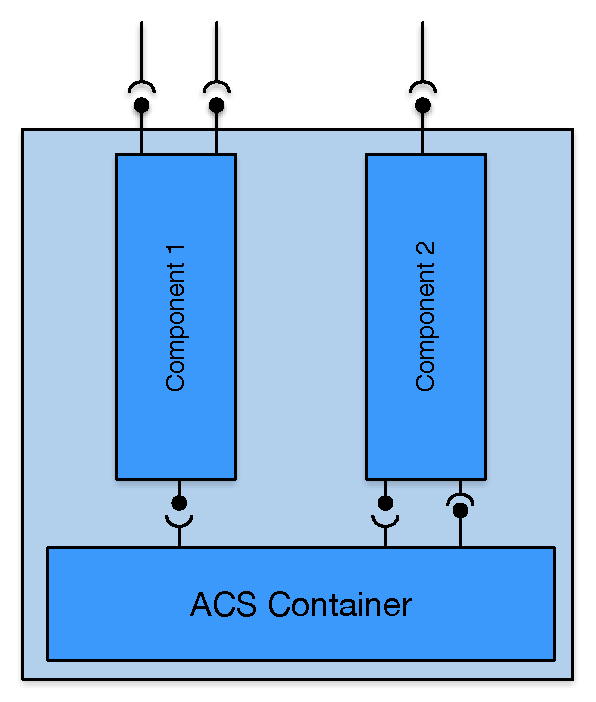
\includegraphics[height=6.8cm]{container_component_corba}
\caption{ACS Container/Component Model}
\end{figure}
\end{frame}


\begin{frame}{Logging System}
\begin{figure}
\centering
	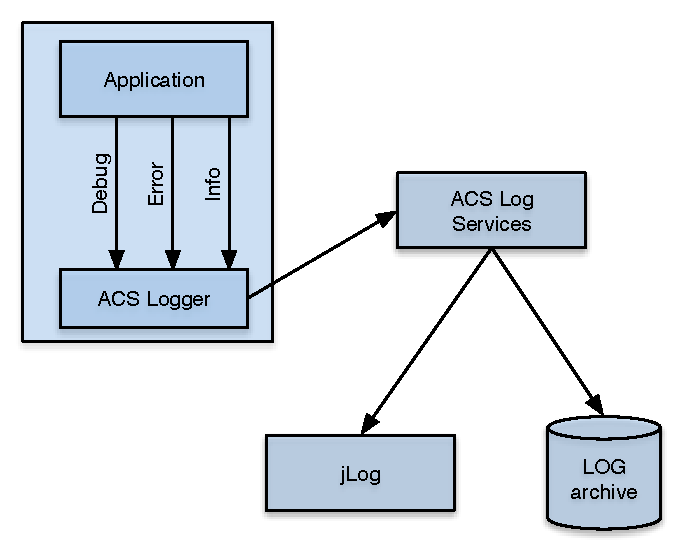
\includegraphics[height=6.8cm]{acs-logging-system}
\caption{ACS Logging system}
\end{figure}
\end{frame}


\begin{frame}[fragile]{Logs}
\begin{lstlisting}[caption=Ejemplo un evento XML de log, language=XML]
<Debug TimeStamp="2002-10-7T13:44:16.530"
	Host="te1.hq.eso.org"
	Process="baciTestServer"
	Thread="main"
	Context=""
	File="baciTestClassImpl.cpp"
	Line="205"
	Routine="BaciTestClass::~BaciTestClass">
    Great debug message!
</Debug>
\end{lstlisting}
	
\end{frame}

\begin{frame}{Pre-procesamiento}
	\begin{itemize}
		\item Tratamiento de texto para eventos
		\begin{itemize}
			\item Separar atributos de cada evento.
			\item Remover números en los mensajes.
			\item Eliminar atributos vacíos.
			\item Transformar el tiempo a formato UNIX
			\item \textit{Stemming} de palabras, (reducción a a la raíz de las palabras)
			\item Eliminación de conectores en mensajes.
		\end{itemize}
		\item Clustering
		\begin{itemize}
			\item Distancia de Levenshtein
			\item Kmeans - IDF
			\item Locality-sensitive hashing algorithms
		\end{itemize}
	\end{itemize}
\end{frame}


\begin{frame}{Procesamiento}
	\begin{itemize}
		\item SVM
	\end{itemize}
	
	\begin{figure}
	\centering
	\begin{tabular}{ l r }
  		
\includegraphics[height=4.5cm]{SVM_margins} &  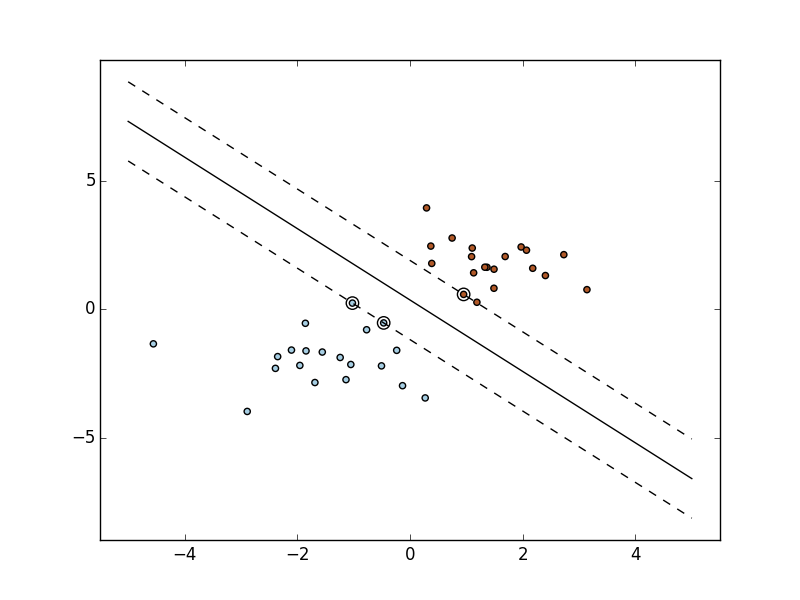
\includegraphics[height=4.5cm]{SVM_plot_sep} \\
	\end{tabular}
	\caption{SVM: Margen de separación}
	
	\end{figure}
\end{frame}

\section{Metodología}
\begin{frame}{CRISP}
\begin{figure}
\centering
	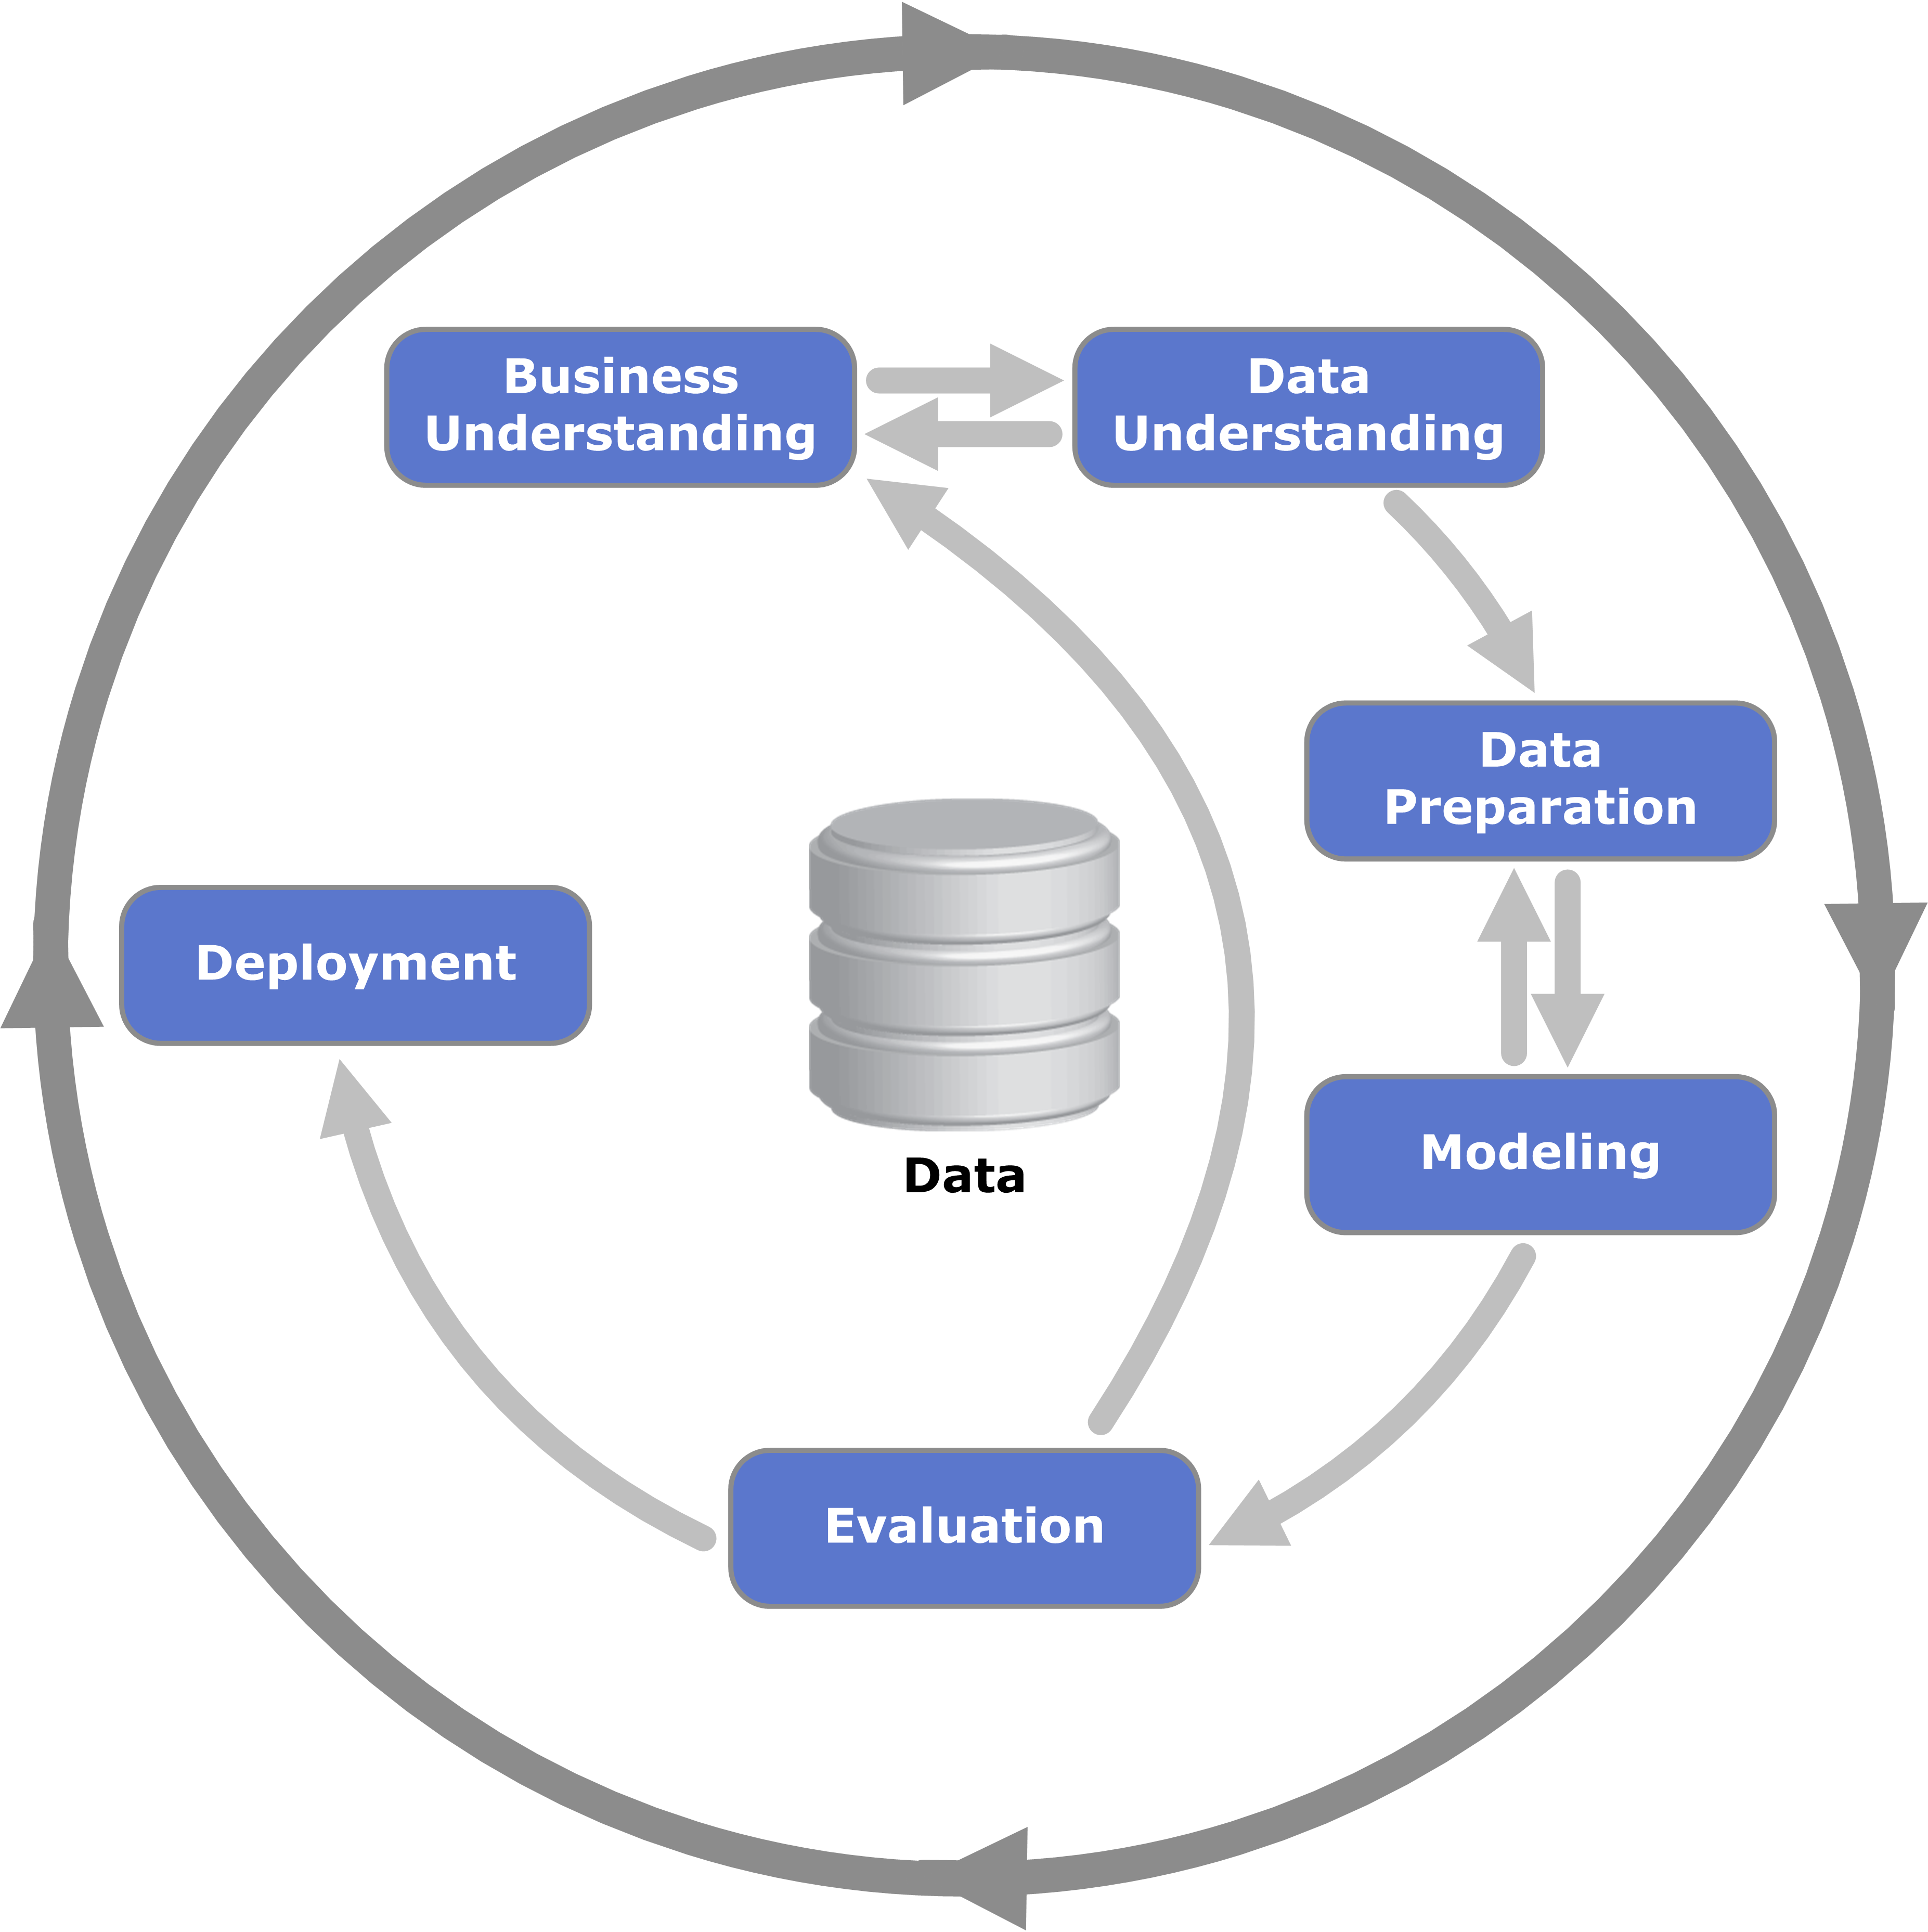
\includegraphics[height=5cm]{crisp}
	\caption{Proceso CRISP}	
\end{figure}
\end{frame}

\section{Programa de trabajo}
\begin{frame}{Programa}
	\begin{enumerate}
	\item Identificar en conjunto con el experto de ALMA una problemática contingente al análisis de logs.

	\item Definir los requisitos del problema identificado.

	\item En conjunto con el experto de ALMA, establecer características relevantes en los patrones de LOGs.
	
	\item Implementar una herramienta para la representación visual de las secuencias de log.

	\item Abordar la problemática utilizando la literatura relacionada con el tema de análisis de logs.
	
\end{enumerate}

\end{frame}
\begin{frame}{Programa}
	\begin{enumerate}
	 \setcounter{enumi}{5}

	\item Identificar una técnica adecuada para enfrentar la problemática.
	
	\item Desarrollar un proceso reducido de \textbf{KDD}, sin iteraciones, basándose en la técnica previamente seleccionada.
	\begin{enumerate}
		\item Selección de un set de datos y operaciones de pre-procesamiento sobre los mismos.
		\item Extracción de características de las secuencias.
		\item Procesamiento de los datos.
		\item Validación de los resultados.
	\end{enumerate}
	\item Elaboración del proyecto.
\end{enumerate}
\end{frame}

\begin{frame}{Carta Gantt}
	\begin{figure}
		\centering
		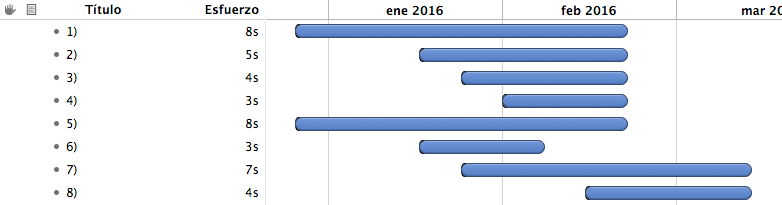
\includegraphics[height=2.5cm]{gantt}
		\caption{Carta Gantt}
	\end{figure}
\end{frame}

\begin{frame}{Preguntas}
\titlepage
\end{frame}

\end{document}